%===============================================================================
% $Id: ifacconf.tex 19 2011-10-27 09:32:13Z jpuente $  
% Template for IFAC meeting papers
% Copyright (c) 2007-2008 International Federation of Automatic Control
%===============================================================================
\documentclass{ifacconf}

\usepackage{graphicx}      % include this line if your document contains figures
\usepackage{natbib}        % required for bibliography
%===============================================================================
\begin{document}
\begin{frontmatter}

\title{Deep Learning for Model-Free Prediction of  Thermal States of Robot Joint Motors} 
% Title, preferably not more than 10 words.

%\thanks[footnoteinfo]{Sponsor and financial support acknowledgment
%goes here. Paper titles should be written in uppercase and lowercase
%letters, not all uppercase.}

\author[First]{Trung Kien La} 
\author[First]{Eric Guiffo Kaigom} 
% \author[Third]{Third C. Author}

\address[First]{Department of Computer Science \& Engineering,
Frankfurt University of Applied Sciences, 60318 Frankfurt am Main, Germany (e-mails: trung.la@stud.fra-uas.de; kaigom@fb2.fra-uas.de).}
% \address[Second]{Colorado State University, 
%    Fort Collins, CO 80523 USA (e-mail: author@lamar. colostate.edu)}
% \address[Third]{Electrical Engineering Department, 
%    Seoul National University, Seoul, Korea, (e-mail: author@snu.ac.kr)}

\begin{abstract}                % Abstract of not more than 250 
	In this work, deep neural networks made up of multiple hidden Long Short-Term Memory (LSTM) and Feed Forward layers are trained to predict the  thermal behavior of the joint motors of robot manipulators. A model-free approach  is adopted. It allows for the accommodation of  complexity and uncertainty challenges that might compromise the derivation, identification, and validation of a large number of  parameters of an approximation model that is hardly available. To this end, sensed joint torques are  collected  and processed  to foresee the thermal behavior of joint motors. Promising prediction results of the machine learning based capture of the temperature dynamics of joint motors of a redundant robot with seven joints are presented. 
\end{abstract}

\begin{keyword}
Robotics, Thermal Management, Artificial Intelligence $\slash$ Machine Learning.
\end{keyword}

\end{frontmatter}
%===============================================================================

\section{Introduction}
Robots are commonly used to unrelentingly achieve repetitive and hazardous tasks in industry and society. Meanwhile, they increasingly and skillfully assist and augment humans. Included are dynamic applications with a pronounced level of physical interactions between humans and robots, such as using a robot as a companion (\cite{basha2025robotic}), home-helper and caregiver (\cite{tsui2025exploring},\cite{gkiolnta2025challenges}), as well as a prosthesis (\cite{kim2025mode}). In this respect, large joint accelerations, high payload manipulations, and motions with specific configurations (see, e.g., Fig. \ref{fig:intro}) can induce an overheating of  joint motors of robots. An excessive motor temperature can accelerate the degradation of insulation materials and reduce the motor efficiency (\cite{yehorov2025study}) along with jeopardizing the positioning accuracy of the robot because of axial  deformations and drifts (\cite{soga2024skillful}). 



Most robot manufacturers, including Franka, Kinova, and KUKA, offer built-in functions to shut down the robot once a critical temperature threshold is attained. Whereas this functionality is advantageous to preserve the performance and reliability of motors and surrounding electronic components, an undesired shutdown is likely to compromise the robot availability for production and assistance purposes. This situation gets exacerbated as the robot is not equipped with mechanical breaks as in Fig. \ref{fig:intro}. In this case, critical collisions with the environment might occur, endangering human beings or leading to hardware (i.e., robot, workpiece, workcell, etc) damages. Furthermore, thermal burns represent  not only  a severe safety issue in physical human-robot-interaction but also a hindrance for elevated user experience that is necessary to engage and sustain a symbiosis between humans and robots.

\begin{figure}[t]
	\centerline{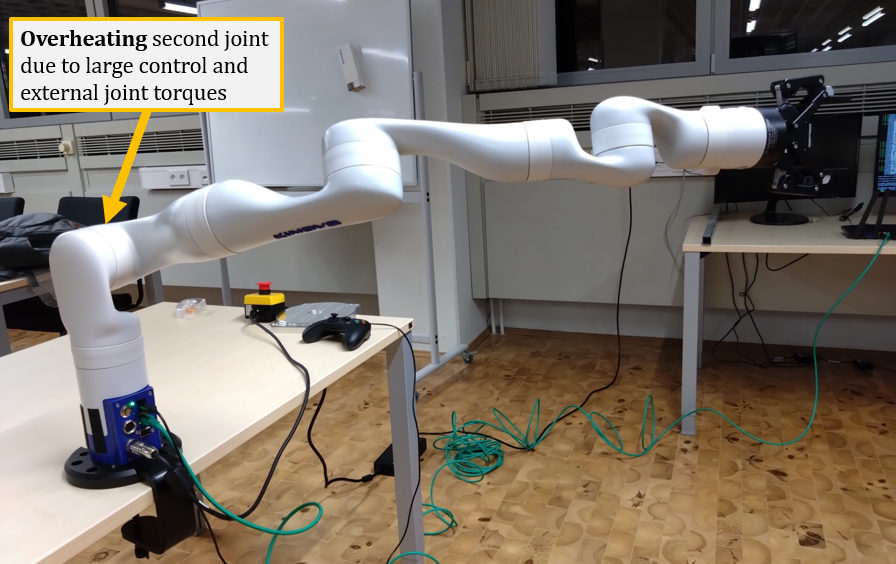
\includegraphics[width=0.97\columnwidth]{pictures/intro.png}}
	\caption{Robot posture increasing a motor temperature.}
	\label{fig:intro}
\end{figure}

Predicting the thermal behavior of robot joints is an essential step toward the development of countermeasures that help anticipate overheating, preserve the robot availability,  prolong its lifetime, and improve its usability. The Industry 4.0, Industry 5.0,  Society 5.0, and Society 6.0 realms are likely to benefit from this capability. This is because it propels operational efficiency through intelligent thermal management of the robot for availability purposes. It also supports decent and sustainable haptic working conditions for the workforce, as well as human-centered robotized servicing for comfortable smart living and social well-being in different ecosystems. Meeting such goals requires an approach that can turn robot diversity and application uncertainties into competitive advantages in terms of flexibility, insights, transferability, and scalability.

This work predicts  the thermal behavior of joint motors of robots with the following key contributions. The prediction approach is
\begin{itemize}
	\item  data-driven, paving the ground for an  insightful, non-invasive, and inclusive operationalization in real-time. The approach therefore follows  design objectives of our overarching Metarobotics framework (\cite{kaigom2023metarobotics}). In our previous work (\cite{abt}), the thermal behavior of  robots is sensed and virtually made accessible to even novices through  immersive, dynamic, and intuitive monitoring and control driven by digital twins (\cite{kaigom2020value}). Since most robots do not output temperature data, we extend our previous work by capturing their thermal motor behavior from observed  actuation profiles.
	\item model-free through the development of a deep learning-based framework that leverages multiple hybrid layers to learn the underlying thermal dynamics of joints from sensed data commonly available via  application programming interfaces (APIs). It is worth noting that no system-related parametric or actuation profile assumptions are made. These particularities are useful to avoid model complexity while fostering generalization and transferability to other robot types regardless of the number and type of joint motors.
	\item evaluated on data collected from a redundant robot with seven joints.
\end{itemize}



\section{Related Works}

Predicting the temperature behavior of robot motors has attracted attention in the recent years.  Online learning of thermal model parameters of a such motor is carried out in \cite{kawaharazuka2020estimation}. The goal is a precise forecasting  of the motor core
temperature of musculoskeletal humanoid robots. An enhanced model allows to predict  maximum output motor torques. Anomalous behaviors are detected by analyzing variations of  thermal dynamics. Thermal control is developed to limit the tensions in the actuation of the musculoskeletal humanoid. In order to safely operate a motor at torques which are considerably larger than its rated torques, \cite{singh2021thermal} capture and regulate  core temperatures via current control. To this end, a thermal abstraction  model is developed and employed to design the thermal controller. The goal is to keep the stator temperature below a heating threshold while avoiding risks of high torques. A method is proposed to control the maximum limit of the current to this end. A forced cooling approach is applied to influence the thermal resistance, steady-state current, and output torque. However, cooling strategies might be challenging to implement once the robot is in use potentially in  toughly accessible environments (e.g., space orbits). In this case, intelligent thermal management approaches are helpful.

\cite{afaq2023intelligent} focus on thermal management of robotic applications under extreme temperatures. Electronics heating and cooling are considered. A temperature control driven by fuzzy logic is developed and demonstrated to this end. Decreases of extreme high temperature from $50^{\circ}$ to $8^{\circ}$ are shown. Fan-based forced convection is used to cool electronics. Excessive internal temperatures in a permanent magnet synchronous motor (PMSM) taking non-stationary loads, which might lead to a reduction of its life time, is addressed in \cite{chen2024lifetime}. An accelerated degradation model is derived to evaluate the reliability function and predict the lifetime of the PMSM under thermal stress.  Geometric backlash and temperature-related drift errors in joints of industrial robots are compensated in \cite{sigron2023compensation}. A model that reflects the thermal expansion of links is developed and used for thermal expansion correction.  LSTM Neural
Networks (\cite{he2024rotor})  and   Pseudo-Siamese Nested LSTM (\cite{cai2021temperature}) are employed to predict the temperature in Permanent Magnet Synchronous Motors. A trapezoidal torque profile is employed in \cite{he2024rotor} whereas the torque dynamics is not released in (\cite{cai2021temperature}). A thermal recovery of robot joints is achieved in  \cite{jorgensen2019thermal}. To this end, the thermal dynamics is captured as a first order ordinary differential equation subject to constant positive and negative step-like profiles of joint torques. The exponential-based dynamics of the temperature behavior is derived.  A parameter identification is carried out to demonstrate the performance of the model for step-like joint torques. Another model-based approach is proposed in \cite{trinh2023modeling} to predict temperature-dependent joint frictions in industrial robots.

Contributions mentioned thus far are mostly model-driven. They fit  with specific robots provided that parameters have been  identified in advance. However, parameter identification requires   noise robustness and low  sensitivity (\cite{zhang2024model}, \cite{de2024non}), which might be a time consuming analysis task  prone to additional uncertainties due to unseen$\slash$unmodeled$\slash$truncated dynamics (\cite{shang2024general}). Sometimes, such a process must  be repeated from scratch for a given new robot, which inhibits quick and large scale automation involving multiple robots in terms of complexity, workload, and costs. As the robot is hardly accessible, such as in space servicing,  identification tasks might be hard to complete because of limited access to pertinent (e.g., excitation) data. Autonomous task completion without human interventions, as expected by Industry 6.0, calls for machine learning-embedded solutions (\cite{carayannis2024toward}) that can extend the robot intelligence for self-condition monitoring. The approach proposed in this work also falls into this category. Robot datasets available from standard APIs are harnessed to predict the thermal behavior of its joint motors. Trained machine learning models can be executed by dedicated services of  digital twins with the physical robot is embedded to detect, communicate to other entities, and anticipate  detrimental thermal issues. In contrast to related works, no restriction is made  on  types of robot, number of joints, and profiles of actuation.

\section{Data-driven prediction of  thermal joint states}

For submission guidelines, follow instructions on paper submission
system as well as the event website.

Note that the $8^{\mathrm{th}}$ IFAC Symposium on Mechatronic Systems and $11^{\mathrm{th}}$ IFAC Symposium on Nonlinear Control Systems impose a strict page limit of 6 pages for full contributions, so it will be better for you to prepare your initial submission in the camera ready layout so that you will have a good estimate for the paper length. Additionally, the effort required for final submission will be minimal.

\subsection{Equations}

Some words might be appropriate describing equation~(\ref{eq:sample}), if 
we had but time and space enough. 

\begin{equation} \label{eq:sample}
{{\partial F}\over {\partial t}} = D{{\partial^2 F}\over {\partial x^2}}.
\end{equation}

See \cite{Abl:56}, \cite{AbTaRu:54}, \cite{Keo:58} and \cite{Pow:85}.

\subsubsection{Example.} This equation goes far beyond the
celebrated theorem ascribed to the great Pythagoras by his followers.

\begin{thm}   % use the thm environment for theorems
The square of the length of the hypotenuse of a right triangle equals
the sum of the squares of the lengths of the other two sides.
\end{thm}

\begin{pf}    % and the pf environment for proofs
The square of the length of the hypotenuse of a right triangle equals the sum of the squares 
of the lengths of the other two sides.
\end{pf}

%% There are a number of predefined theorem-like environments in
%% ifacconf.cls:
%%
%% \begin{thm} ... \end{thm}            % Theorem
%% \begin{lem} ... \end{lem}            % Lemma
%% \begin{claim} ... \end{claim}        % Claim
%% \begin{conj} ... \end{conj}          % Conjecture
%% \begin{cor} ... \end{cor}            % Corollary
%% \begin{fact} ... \end{fact}          % Fact
%% \begin{hypo} ... \end{hypo}          % Hypothesis
%% \begin{prop} ... \end{prop}          % Proposition
%% \begin{crit} ... \end{crit}          % Criterion

Of course LaTeX manages equations through built-in macros. You may
wish to use the \texttt{amstex} package for enhanced math
capabilities.

\subsection{Figures}

To insert figures, use the \texttt{graphicx} package. Although other
graphics packages can also be used, \texttt{graphicx} is simpler to
use. See  Fig.~\ref{fig:bifurcation} for an example.

\begin{figure}
\begin{center}
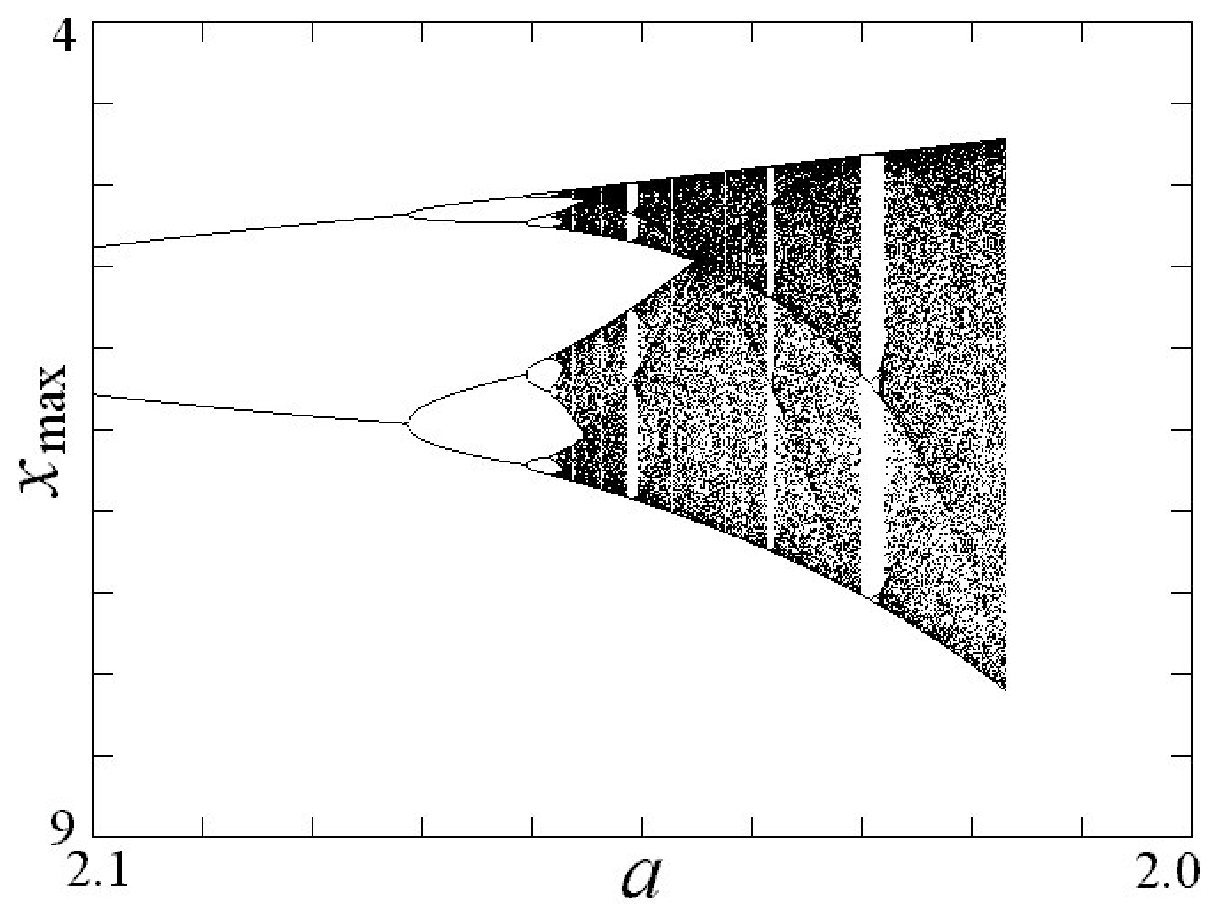
\includegraphics[width=8.4cm]{bifurcation}    % The printed column width is 8.4 cm.
\caption{Bifurcation: Plot of local maxima of $x$ with damping $a$ decreasing} 
\label{fig:bifurcation}
\end{center}
\end{figure}

Figures must be centered, and have a caption at the bottom. 

\subsection{Tables}
Tables must be centered and have a caption above them, numbered with
Arabic numerals. See table~\ref{tb:margins} for an example.

\begin{table}[hb]
\begin{center}
\caption{Margin settings}\label{tb:margins}
\begin{tabular}{cccc}
Page & Top & Bottom & Left/Right \\\hline
First & 3.5 & 2.5 & 1.5 \\
Rest & 2.5 & 2.5 & 1.5 \\ \hline
\end{tabular}
\end{center}
\end{table}

\subsection{Final Stage}

Authors are expected to mind the margins diligently.  Papers need to
be stamped with event data and paginated for inclusion in the
proceedings. If your manuscript bleeds into margins, you will be
required to resubmit and delay the proceedings preparation in the
process.

\subsubsection{Page margins.} See table~\ref{tb:margins} for the
page margins specification. All dimensions are in \emph{centimeters}.


\subsection{PDF Creation}

All fonts must be embedded/subsetted in the PDF file. Use one of the
following tools to produce a good quality PDF file:

\subsubsection{PDFLaTeX} is a special version of LaTeX by Han The
Thanh which produces PDF output directly using Type-1 fonts instead of
the standard \texttt{dvi} file. It accepts figures in JPEG, PNG, and PDF
formats, but not PostScript. Encapsulated PostScript figures can be
converted to PDF with the \texttt{epstopdf} tool or with Adobe Acrobat
Distiller.

\subsubsection{Generating PDF from PostScript} is the classical way of
producing PDF files from LaTeX. The steps are:

\begin{enumerate}
  \item Produce a \texttt{dvi} file by running \texttt{latex} twice.
  \item Produce a PostScript (\texttt{ps}) file with \texttt{dvips}.
  \item Produce a PDF file with \texttt{ps2pdf} or Adobe Acrobat
  Distiller.
\end{enumerate}

\subsection{Copyright Form}

IFAC will put in place an electronic copyright transfer system in due
course. Please \emph{do not} send copyright forms by mail or fax. More
information on this will be made available on IFAC website.

\section{Data Acquisition and Preprocessing}
- Kinova Gen3 7 DoF Robot \\
- OPC UA Server and Client (data: pos, temp, torques, velocities and current), create Figure\\
- randomly generated (restrcited) joint angles/trajectories \\
- (reference to streamlit app?)\\
- Fit function with collected data? \\
- description of data preprocessing for LSTM and FF

\begin{figure}
  \begin{center}
  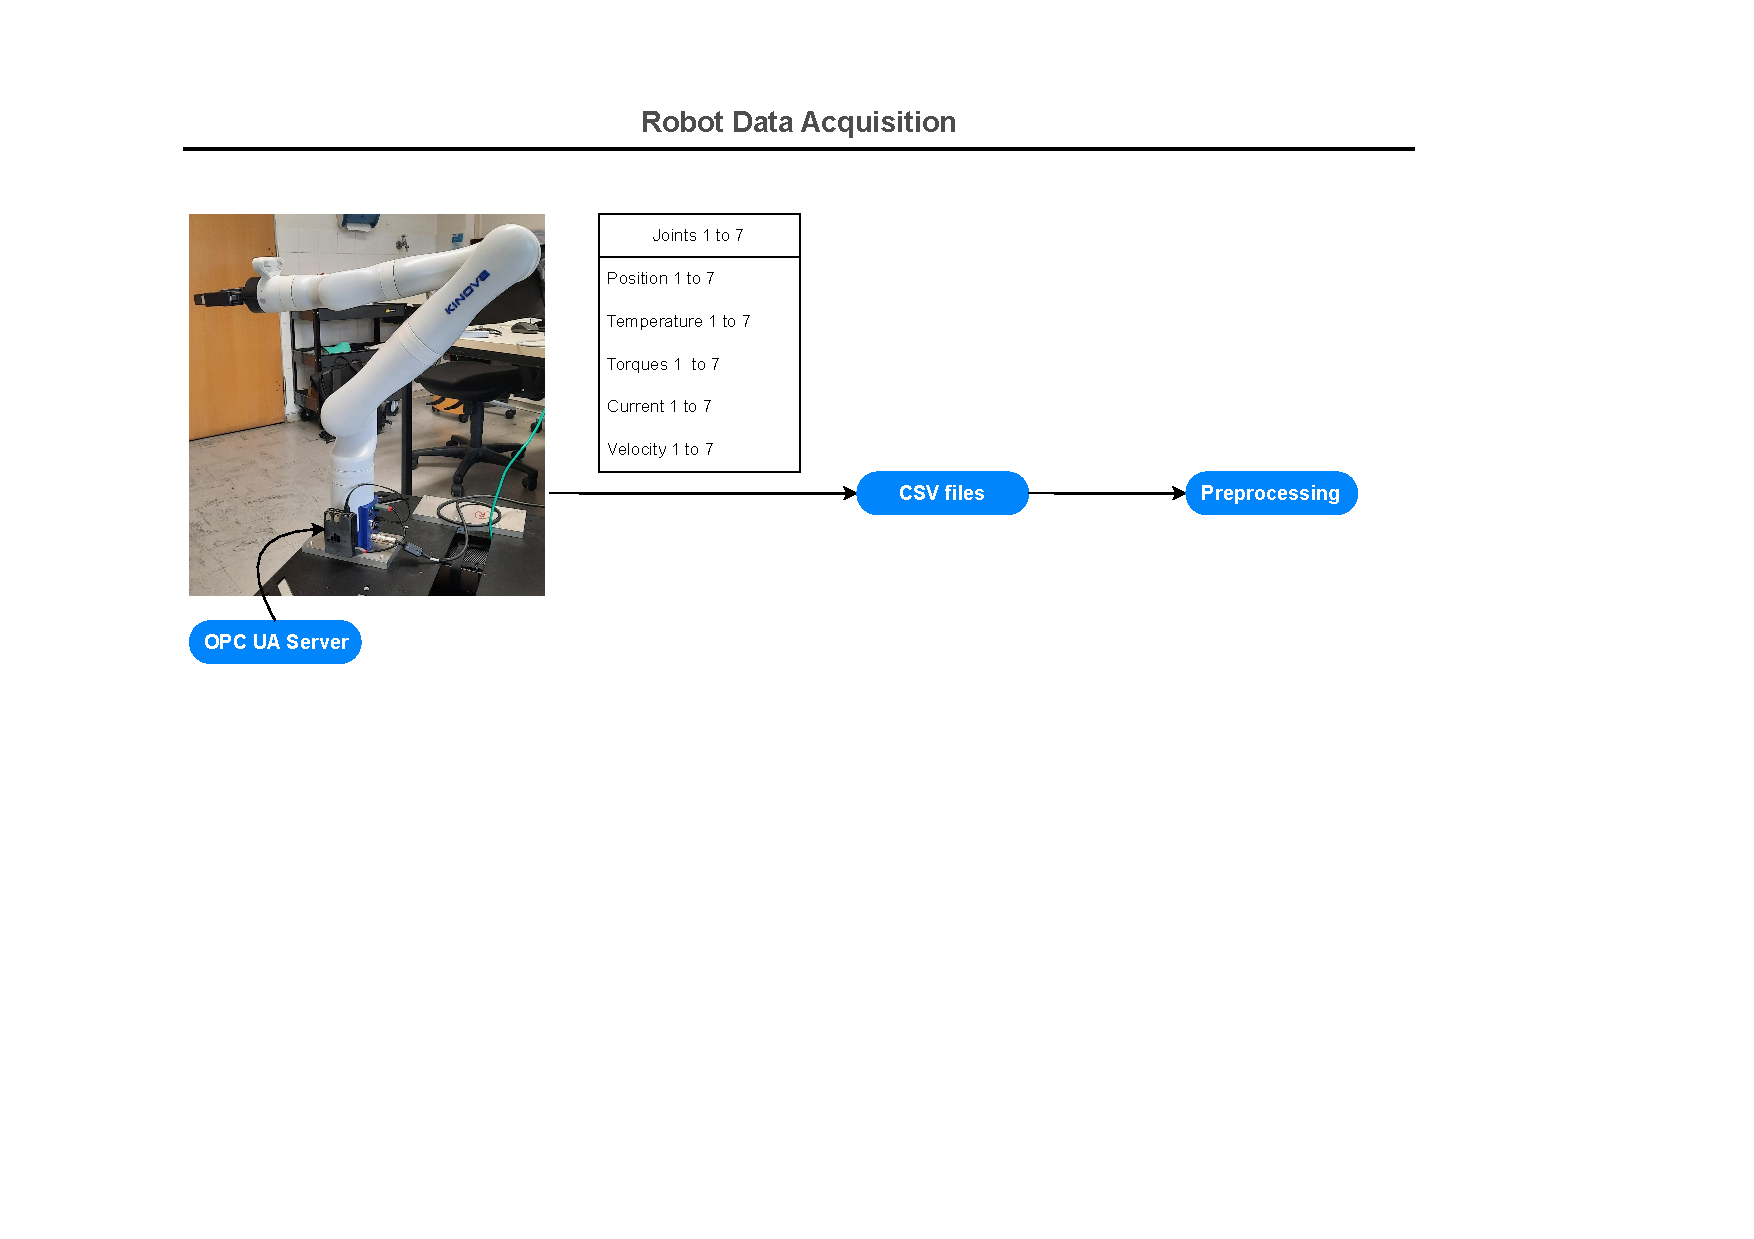
\includegraphics[width=8.4cm]{pictures/DataAquisition.pdf}    % The printed column width is 8.4 cm.
  \caption{Kinova data aquisition via OPC UA Server} 
  \label{fig:DataAquisition}
  \end{center}
  \end{figure}


% \section{Units}

% Use SI as primary units. Other units may be used as secondary units
% (in parentheses). This applies to papers in data storage. For example,
% write ``$15\,\mathrm{Gb}/\mathrm{cm}^2$ ($100\,\mathrm{Gb}/\mathrm{in}^2$)''. 
% An exception is when
% English units are used as identifiers in trade, such as ``3.5 in
% disk drive''. Avoid combining SI and other units, such as current in
% amperes and magnetic field in oersteds. This often leads to confusion
% because equations do not balance dimensionally. If you must use mixed
% units, clearly state the units for each quantity in an equation.  The
% SI unit for magnetic field strength $\mathbf{H}$ is $\mathrm{A}/\mathrm{m}$. However, if you wish to
% use units of $\mathrm{T}$, either refer to magnetic flux density $\mathbf{B}$ or
% magnetic field strength symbolized as $\mu_0\,\mathbf{H}$. Use the center dot to
% separate compound units, e.g., ``$\mathrm{A} \cdot \mathrm{m}^2$''.

\section{Proposed Models (various LSTMs, FeedForward) [and Comparision?]}
- various LSTMs (Strcuture: Hyperparameter {Learning Rate, Epochs, Batch Size, no. of Layers, Regularization, adam optimization}, RMSE, True vs Predicted Temps, etc.)\\
- FeedForward (same as above)\\
- fitted function?\\
- Comparisions

\subsection{Figures and Tables}

Figure axis labels are often a source of confusion. Use words rather
than symbols. As an example, write the quantity ``Magnetization'', or
``Magnetization M'', not just ``M''. Put units in parentheses. Do not
label axes only with units.  For example, write ``Magnetization
($\mathrm{A}/\mathrm{m}$)'' or ``Magnetization ($\mathrm{A} \mathrm{m}^{-1}$)'', not just
 ``$\mathrm{A}/\mathrm{m}$''. Do not
label axes with a ratio of quantities and units. For example, write
``Temperature ($\mathrm{K}$)'', not ``$\mbox{Temperature}/\mathrm{K}$''.

Multipliers can be especially confusing. Write ``Magnetization
($\mathrm{kA}/\mathrm{m}$)'' or ``Magnetization ($10^3 \mathrm{A}/\mathrm{m}$)''. Do not write
``Magnetization $(\mathrm{A}/\mathrm{m}) \times 1000$'' because the reader would not know
whether the axis label means $16000\,\mathrm{A}/\mathrm{m}$ or $0.016\,\mathrm{A}/\mathrm{m}$.

\subsection{References}

Use Harvard style references (see at the end of this document). With
\LaTeX, you can process an external bibliography database 
using \texttt{bibtex},\footnote{In this case you will also need the \texttt{ifacconf.bst}
file, which is part of the \texttt{ifaconf} package.}
or insert it directly into the reference section. Footnotes should be avoided as
far as possible.  Please note that the references at the end of this
document are in the preferred referencing style. Papers that have not
been published should be cited as ``unpublished''.  Capitalize only the
first word in a paper title, except for proper nouns and element
symbols.

\subsection{Abbreviations and Acronyms}

Define abbreviations and acronyms the first time they are used in the
text, even after they have already been defined in the
abstract. Abbreviations such as IFAC, SI, ac, and dc do not have to be
defined. Abbreviations that incorporate periods should not have
spaces: write ``C.N.R.S.'', not ``C. N. R. S.'' Do not use abbreviations
in the title unless they are unavoidable (for example, ``IFAC'' in the
title of this article).

\subsection{Equations}

Number equations consecutively with equation numbers in parentheses
flush with the right margin, as in (\ref{eq:sample}).  To make your equations more
compact, you may use the solidus ($/$), the $\exp$ function, or
appropriate exponents. Use parentheses to avoid ambiguities in
denominators. Punctuate equations when they are part of a sentence, as
in

\begin{equation} \label{eq:sample2}
\begin{array}{ll}
\int_0^{r_2} & F (r, \varphi ) dr d\varphi = [\sigma r_2 / (2 \mu_0 )] \\
& \cdot \int_0^{\inf} exp(-\lambda |z_j - z_i |) \lambda^{-1} J_1 (\lambda  r_2 ) J_0 (\lambda r_i ) d\lambda 
\end{array}
\end{equation}

Be sure that the symbols in your equation have been defined before the
equation appears or immediately following. Italicize symbols ($T$
might refer to temperature, but T is the unit tesla). Refer to
``(\ref{eq:sample})'', not ``Eq. (\ref{eq:sample})'' or ``equation
(\ref{eq:sample})'', except at the beginning of a sentence: ``Equation
(\ref{eq:sample}) is \ldots''.

\subsection{Other Recommendations}

Use one space after periods and colons. Hyphenate complex modifiers:
``zero-field-cooled magnetization''. Avoid dangling participles, such
as, ``Using (1), the potential was calculated'' (it is not clear who or
what used (1)). Write instead: ``The potential was calculated by using
(1)'', or ``Using (1), we calculated the potential''.

A parenthetical statement at the end of a sentence is punctuated
outside of the closing parenthesis (like this). (A parenthetical
sentence is punctuated within the parentheses.) Avoid contractions;
for example, write ``do not'' instead of ``don' t''. The serial comma
is preferred: ``A, B, and C'' instead of ``A, B and C''.
\section{Discussion?}
?
\section{Conclusion}

A conclusion section is not required. Although a conclusion may review
the main points of the paper, do not replicate the abstract as the
conclusion. A conclusion might elaborate on the importance of the work
or suggest applications and extensions.

\begin{ack}
Place acknowledgments here.
\end{ack}

\bibliography{ifacconf}             % bib file to produce the bibliography
                                                     % with bibtex (preferred)
                                                   
%\begin{thebibliography}{xx}  % you can also add the bibliography by hand

%\bibitem[Able(1956)]{Abl:56}
%B.C. Able.
%\newblock Nucleic acid content of microscope.
%\newblock \emph{Nature}, 135:\penalty0 7--9, 1956.

%\bibitem[Able et~al.(1954)Able, Tagg, and Rush]{AbTaRu:54}
%B.C. Able, R.A. Tagg, and M.~Rush.
%\newblock Enzyme-catalyzed cellular transanimations.
%\newblock In A.F. Round, editor, \emph{Advances in Enzymology}, volume~2, pages
%  125--247. Academic Press, New York, 3rd edition, 1954.

%\bibitem[Keohane(1958)]{Keo:58}
%R.~Keohane.
%\newblock \emph{Power and Interdependence: World Politics in Transitions}.
%\newblock Little, Brown \& Co., Boston, 1958.

%\bibitem[Powers(1985)]{Pow:85}
%T.~Powers.
%\newblock Is there a way out?
%\newblock \emph{Harpers}, pages 35--47, June 1985.

%\bibitem[Soukhanov(1992)]{Heritage:92}
%A.~H. Soukhanov, editor.
%\newblock \emph{{The American Heritage. Dictionary of the American Language}}.
%\newblock Houghton Mifflin Company, 1992.

%\end{thebibliography}

\appendix
\section{A summary of Latin grammar}    % Each appendix must have a short title.
\section{Some Latin vocabulary}              % Sections and subsections are supported  
                                                                         % in the appendices.
\end{document}
